\chapter[Estrutura]{Estrutura}
	
	A estrutura física do R.I.C.C. é composta de uma estação que integra o sistema energético Off-Grid e os equipamentos eletrônicos de processamento e transmissão, uma régua de medição equipada com os sensores de solo acoplada à estação, além de estruturas auxiliares. O design de cada módulo será feito com base nos elementos elétricos e eletrônicos utilizados.
	
	O trabalho inicial concentra-se na análise do levantamento de requisitos do projeto, elaborando um modelo que atenda as solicitações de cada subsistema. O projeto estrutural deve: $(1)$ Fornecer sustentação aos componentes de cada subsistema, de acordo com sua operação, posicionamento e dimensões, $(2)$ Ser pensado de modo a facilitar a atuação de cada componente, $(3)$ Ter sua utilização da forma mais prática possível. O projeto estrutural não será definido antes do levantamento dos componentes internos, visando uma construção que atenda os subsistema de forma adequada.
	
	\section{Estação}
	
	A estação será a estrutura em campo que deve conter os sistemas eletrônicos de medição de informações atmosféricas (Umidade, temperatura, velocidade do vento, irradiação solar e pluviosidade), de processamento dos sinais adquiridos pela régua e de transmissão de sinal, além de um sistema de alimentação fotovoltaico independente. Será capaz de proteger os componentes sensíveis de jatos d’água provenientes de chuva e irrigação e do aquecimento devido a irradiação solar, de ficar fixa ao solo e não ser danificada independente da ação do vento, de permitir a escolha de altura e a fixação da inclinação da placa solar facilmente pelo operador. 
	
	Considera-se então a ideia inicial de uma estrutura modular de seção quadrada, construída com longarinas metálicas e coberta por placas de fibra de vidro que separariam cada seção e as isolaria do meio externo conforme os requisitos apresentados. Dessa forma, é possível construir um produto leve, de resistência mecânica adequada, que confira fácil acesso a todos os componentes internos, apesar de protegê-los, com estética simples, mas elegante, além de garantir manufatura, montagem e armazenamento facilitados, bem como uma boa durabilidade.
	
	\begin{figure}[H]
	\centering
	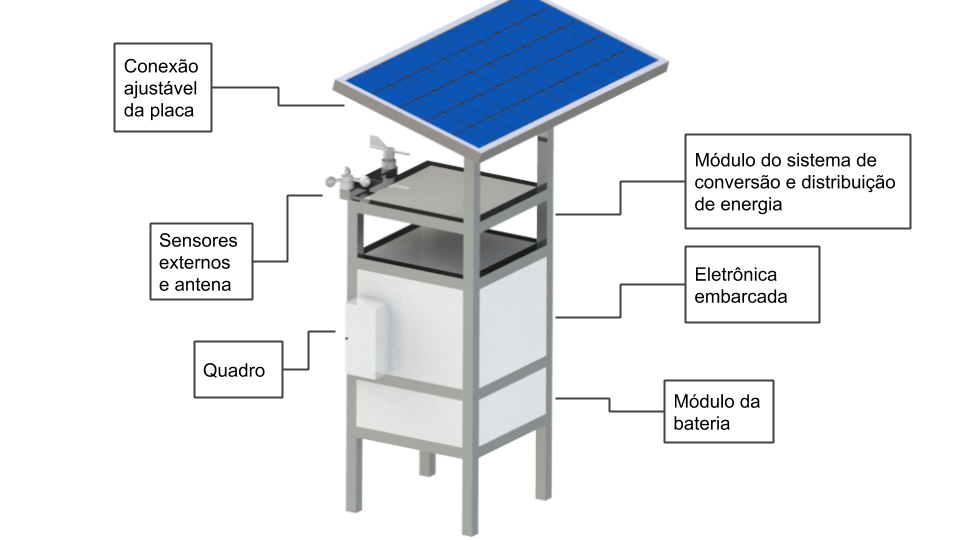
\includegraphics[width=0.8\linewidth]{estrutura/figuras/est_pc1_01_estacao.png}
  	\caption{Design inicial da estação}
  	\label{Estação}
	\end{figure}
	
	A estação se organiza em 3 módulos internos. O módulo inferior é dedicado exclusivamente para a bateria, será fechado e a prova de aguá. Por ser o elemento mais pesado da estação e também mais caro, seu módulo exclusivo posicionará a bateria da melhor maneira para sua proteção e pleno funcionamento.
	
	O módulo acima deste abriga a maior parte dos componentes internos da estação, nele se desenvolve o ajuste da energia captada pelo painel até a utilização nos componentes eletrônicos. Este módulo também é protegido da água e da irradiação solar. No lado externo deste módulo localiza-se um quadro de distribuição de fácil acesso, não sendo necessário a abertura da estrutura para manuseá-lo.
	
	O módulo superior abriga o sistema eletrônico embarcado que é uma fonte de calor intensa, por isto este módulo será aberto para trocas de calor com ambiente, mas protegido da água. Esta configuração foi pensada pela existência do cooler para refrigeração da placa, assim sendo, o calor retirado da placa não é contido na estrutura, mas trocado com o ambiente.
	
	Na parte superior da estrutura posicionam-se os sensores atmosféricos (Velocidade do vento, temperatura ambiente, pluviosidade, irradiação solar UV), a antena para transmissão dos dados e o painel fotovoltaico que gera energia para o sistema. Os sensores são posicionados de forma que o painel não influencie as medições, já o painel terá um ajuste manual de inclinação, com um grau de liberdade. 
	
	
	\subsection{Controle de Temperatura}
	Uma das preocupações centrais do projeto está relacionada com o controle térmico dos componentes da estação, tendo em vista a exposição da estrutura a irradiação solar e ainda a potência dissipada por componentes eletrônicos e do sistema fotovoltaico. Por conta da estrutura modular, estudamos uma solução específica para cada sistema, de acordo com a demanda térmica dos elementos.
 
 Os elementos principais de análise são a bateria, que possui um  módulo próprio na parte inferior da estrutura, e o sistema eletrônico embarcado, que se encontra no primeiro módulo. Para cada um desses elementos pesquisamos as condições de funcionamento adequadas e pensamos em soluções específicas.
 
\subsubsection*{Bateria}

 Para preservar a vida útil da bateria fotovoltaica, que junto ao painel solar serão responsáveis pelo abastecimento energético da estação e da régua de sensores, estipulamos a temperatura limite de funcionamento inferior a $40 \degree C$ de acordo com a análise: \cite{Freedom}
 
 Nesse cenário se deve isolar a bateria da irradiação solar. Para isso algumas alternativas foram levantadas considerando prós e contras de execução:
 
\begin{itemize}
\item Revestir o esqueleto estrutural de metal com placas de fibra de vidro, fazendo assim a divisão de módulos do corpo; a fibra de vidro atua como isolante térmico devido a razão elevada de área por massa, apresentando uma condutividade térmica média de $0,05 ~~\sfrac{W}{mK}$, valor próximo de $0$. \label{item1}
\item Aletar a estrutura em torno da bateria para aumentar sua área de contato com o ar ambiente, intensificando assim o efeito dissipador de calor. \label{item2}
\end{itemize} 

 Em relação a primeira solução \ref{item1}, a viabilidade da proposta está de acordo com as demais exigências estruturais, entre elas, garantir que os módulos permaneçam secos e protegidos da água. Já o dimensionamento e a produção de aletas para envelopar a bateria \ref{item2} apresentam grandes dificuldades associadas, prejudicando a  viabilidade da solução e uma vez que uma proteção a irradiação solar é suficiente para manter a bateria em condições normais de funcionamento \cite{Freedom}. Entre as principais dificuldades encontram-se:

\begin{itemize}
\item Estipular parâmetros de controle e modelar o funcionamento térmico das aletas, otimizando a geometria a ser escolhida e os materiais envolvidos.
\item Manufaturar esse elemento estrutural com precisão suficiente para garantir o rendimento teórico dos materiais e da estrutura aletada.
\item Garantir o isolamento da irradiação solar, considerando que o princípio de funcionamento de aletas se baseia na condução e convecção de calor e os efeitos da irradiação poderiam anular as contribuições positivas (retirar calor da fonte quente) e até reverte-las, resultando em um fluxo de calor no sentido da bateria, causando um resultado contrário ao resfriamento desse elemento.  
\end{itemize}


\subsubsection*{Sistema eletrônico embarcado}

 Diferente da bateria, a principal preocupação com esse componente é evitar o superaquecimento, tendo em vista sua temperatura de funcionamento mais elevada. A partir dos $80 \degree C$ esse microcontrolador reduz o \textit{clock} de processamento para evitar superaquecimentos, assim essa será a temperatura limite considerada.
 
 Esse valor elevado justifica o cuidado com os demais elementos e separação da placa em um módulo separado dos demais componentes do módulo eletrônico. A solução adotada se baseou em uma série de testes realizadas com a placa monitorando sua temperatura de funcionamento em diversas configurações distintas.
 
 O modelo da Raspberry Pi 3 possui uma série de acessórios e dispositivos complementares em seu catálogo. Entre eles um \textit{cooler} acoplado a \textit{case} da placa que funciona como um sistema de arrefecimento forçado.
 
 Um estudo de comparação de temperatura com esse acessório, o estabelece como solução viável. Simulando o funcionamento da Raspberry ao longo do tempo, foram obtidos gráficos comparativos da temperatura da placa e ainda foram feitas medições acerca dos arredores da placa.

 \begin{itemize}
 \item Caso 1: funcionamento da placa  com a \textit{case} sem refrigeração forçada:
 \begin{figure}[H]
	\centering
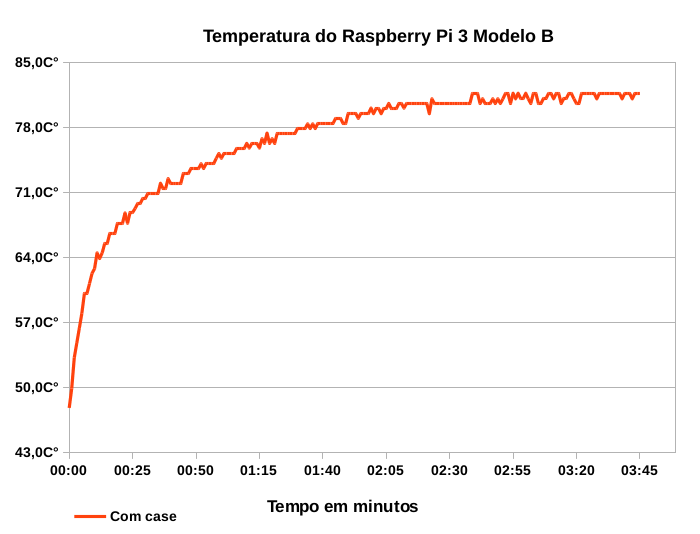
\includegraphics[width=0.8 \textwidth]{estrutura/figuras/temperatura_raspberry_pi_3_grafico_com_case}
	\caption{Evolução de temperatura sem resfriamento. Fonte: \cite{resf_rasp}}
	\label{fig1} 
	\end{figure}

 A temperatura máxima da placa alcançou o patamar de $86 \degree C$ e a \textit{case} chegou a um pico de $44,7 \degree C$.
 
 \item Caso 2: funcionamento da placa com a \textit{case} e o \textit{cooler}: 
 \begin{figure}[H]
	\centering
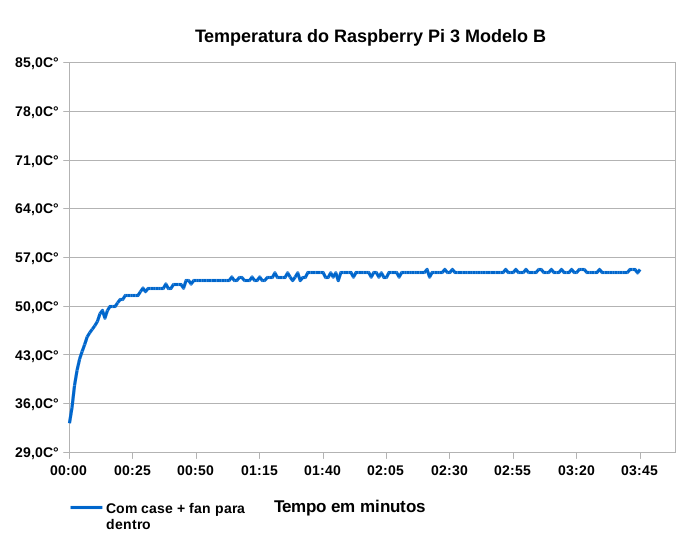
\includegraphics[width=0.8 \textwidth]{estrutura/figuras/temperatura_raspberry_pi_3_grafico_com_case_cooler_dentro}
\caption{Evolução de temperatura com resfriamento. Fonte: \cite{resf_rasp}}
	\label{fig2} 
	\end{figure}

 A temperatura máxima da placa alcançou o patamar de $56,9 \degree C$ e a \textit{case} chegou a um pico de $24 \degree C$. Esses testes foram realizados a temperatura ambiente de $22 \degree C$.
  
 \end{itemize}

	Com a validação desse estudo, partimos para o dimensionamento desse componente. As especificações do produto escolhido são as seguintes: 
	\begin{itemize}
	\item Funcionamento DC
	\item Tensão de operação ($V$): $4,0 \sim 5,75$ 
	\item Corrente ($A$): $0,14 \sim 0,2$
	\item Potência máxima consumida ($W$): $v_{max} \times i_{max} = 1,15$ 
	\end{itemize}

 \begin{figure}[H]
	\centering
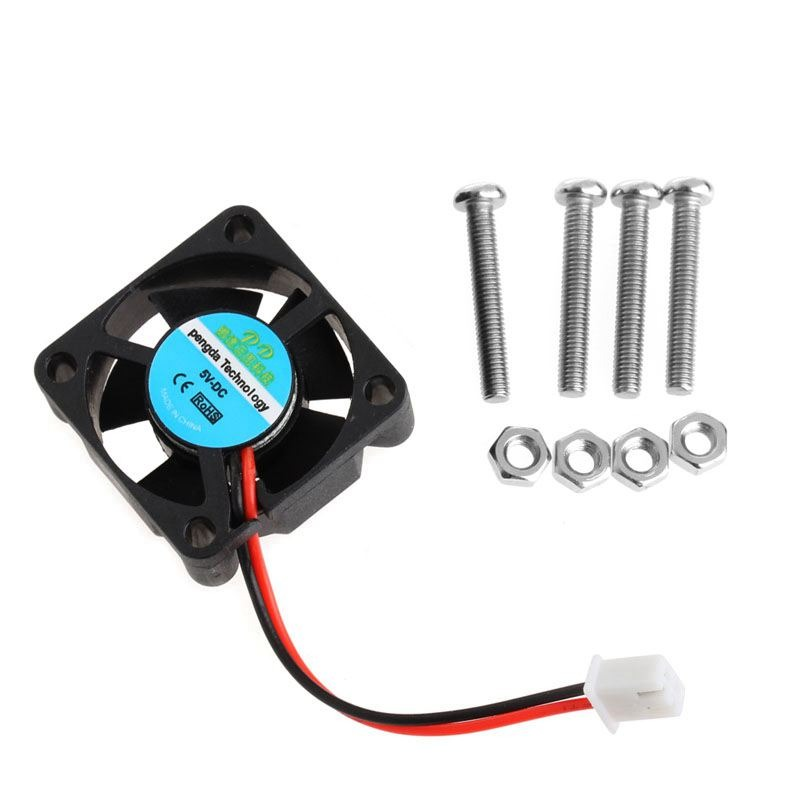
\includegraphics[width=0.4 \textwidth]{estrutura/figuras/cooler}
%	\caption{}
	\label{fig3} 
	\end{figure}
	
	
 	\section{Quadros}
	
	Os quadros para instalações elétricas tem o objetivo de organizar e proteger a distribuição da energia. Eles tem dimensão estimada de $25 \times 19.5 \times 11 cm $ e serão utilizados na estação e no pivô de irrigação.
	São encontrados diversos modelos comerciais, porém é de interesse o design de uma estrutura específica para o nosso projeto. Dessa forma, será possível garantir a alocação adequada dos sistemas com componentes de dimensões apropriadas para o projeto e que sejam visualmente harmoniosos na composição geral. Espera-se utilizar plástico ABS impresso no interior, assim é possível acomodar as peças com segurança para o sistema e para o usuário, além de permitir fácil acesso em caso de manutenção.

	
	\section{Régua de medição}
	
	A régua de medição é a estrutura de acoplagem e proteção dos componentes eletrônicos inseridos no solo, capaz de protegê-los durante a inserção na terra, todo o período de medição e remoção do sistema. Deverá também ser projetada de forma a permitir o posicionamento dos sensores de umidade de solo em diferentes profundidades e manuseio facilitado, sem a necessidade de muitos ajustes pelo operador. Para tanto, espera-se inicialmente utilizar plástico ABS impresso reforçado com longarinas de aço e placas de fibra de vidro, de forma a garantir geometria de precisão suficiente e resistência mecânica adequada. Será possível, portanto, alojar os sensores e resistir à compactação do solo, além de possíveis impactos de ferramentas utilizadas na cultura, em uma estrutura prática. 
	
	\section{Materiais}
	
	A escolha de materiais para a construção da estrutura é parte fundamental do trabalho, pois são as propriedades do material escolhido que dão as características de atuação de nosso projeto. A escolha passa por uma análise dos esforços identificados, facilidade de aquisição, dificuldade de manuseio e o custo do material, além de outros fatores decorrentes do projeto.
	
	Nesta etapa do projeto, diversos materiais são sugeridos e suas propriedades são analisadas com objetivo de realizar a melhor escolha.
	
	
	O \textbf{Aço Carbono} é um material de fácil aquisição no mercado, sobretudo os aços com baixo teor de carbono, além de uma alta soldabilidade e usinabilidade, baixo custo e boa resistência mecânica. Entretanto é facilmente oxidado pelo ar, quando sem revestimento de proteção, e possui uma elevada massa específica.
	
	O \textbf{Aço Inox} já apresenta maior dificuldade de aquisição, devido a um menor número de fornecedores quando comparados ao aço carbono. Apresenta excelente acabamento superficial e maior resistência à corrosão. Possui uma elevada densidade, e requer maiores tecnologias para realizar soldagem e conformação mecânica, além do elevado custo.
	
	O \textbf{Aço Cr-Mo} é uma liga com altíssima resistência mecânica, entretanto apresenta alto custo e baixa usinabilidade. Ainda assim, apresenta uma pequena gama de fornecedores no Brasil.
	
	O \textbf{Alumínio} é um metal muito dúctil, com baixa densidade, boa resistência mecânica e acabamento. A solda deste material é complexa, porém sua versão estrutural tem secção transversal projetada de forma a facilitar encaixes simples e  são encontrados em diversos locais, porém apresentam um custo elevado.\cite{callister}
	
	Construímos uma matriz de decisão com a finalidade de auxiliar na comparação do material a ser empregado no projeto e atribuindo valores de 1 a 10 sendo 10 excelente e 1 péssimo. 
	
\begin{table}[H]
\centering
\caption{Matriz de decisão de materiais}
\begin{tabular}{|c|c|c|c|c|}
\hline
\textbf{Critérios}      & \textbf{Aço Carbono} & \textbf{Aço Inox} & \textbf{Aço Cr-Mo} & \textbf{Alumínio} \\ \hline
Peso                               & 6                    & 6                 & 5                  & 9                 \\ \hline
Preço                              & 9                    & 8                 & 5                  & 5                 \\ \hline
Resistência  Mecânica               & 9                    & 7                 & 10                 & 7                 \\ \hline
Resistência à Corrosão              & 4                    & 8                 & 5                  & 9                 \\ \hline
Soldabilidade                       & 9                    & 7                 & 7                  & 5                 \\ \hline
\end{tabular}
\end{table}

	Além de materiais metálicos, analisamos o uso de polímeros para impressão 3D para confecção de algumas partes do projeto. A impressão possibilita um desenho preciso de peças, de acordo com seu uso.
	
	O PLA possui temperatura de fusão baixa, de $180 \degree C$, e a partir de $60 \degree C$ as moléculas internas começam a se mover e a peça começa a “amolecer”. Isso é ruim se tratando de peças que precisam ser expostas ao sol. É o material que mais suporta desgaste superficial, ou atrito.

	O ABS é o que melhor suporta temperatura entre os materiais aqui avaliados, cerca de $100 \degree C$. Sua dureza superficial baixa em relação aos demais desqualifica-o para utilização em peças que necessitam contato.

 O PETG apresenta boa resistência mecânica, possui uma resistência a temperatura e suporta exposição ao sol ($85 \degree C$). Sua dureza superficial é baixa e é um material muito resistente.
 
 \begin{table}[H]
\centering
\caption{Propriedades dos polímeros para impressão}
\begin{tabular}{|c|c|c|c|}
\hline
\textbf{Critérios}     & \textbf{PLA} & \textbf{ABS} & \textbf{PETG} \\ \hline
Densidade              & 1,24         & 1,04         & 1,27          \\ \hline
Transição Vítrea       & 60           & 100          & 85            \\ \hline
Módulo de elasticidade & 4350         & 2200         & 2120          \\ \hline
Tensão de Escoamento   & 66           & 38           & 51            \\ \hline
\end{tabular}
\end{table}
	
	Com os dados comparativos, podemos fazer uma melhor analise de alguns materiais. Por exemplo, o alumínio estrutura não é uma escolha tão vantajosa devido ao alto custo. No lugar, preferimos utilizar o aço carbono que tem bom custo, pois suas desvantagens (peso e acabamento) não afetam tanto o projeto. 

	  